
\section{Algortihm in CUDA with double precision arithmetic and data types (3/4 Points)}
\subsection{OpenCL Kernel to Compute Dot Product of two vectors}
The given code skelleton \fun{vector\_add.cpp} was adapted in a very rudimentary way without shared memory or any other bamboozles! The Sum of the entries later computed on the CPU.

\begin{lstlisting}[language=C++, title=C++ Code Changes in \fun{vector\_add.cpp}]
const char *my_opencl_program = R"(
#pragma OPENCL EXTENSION cl_khr_fp64 : enable    // required to enable 'double' inside OpenCL programs

__kernel void vec_add(__global double *x,
                      __global double *y,
                      unsigned int N)
{
  for (unsigned int i  = get_global_id(0);
                    i  < N;
                    i += get_global_size(0))
    x[i] = x[i] * y[i];
})"; 


double dot_product = 0;
for(int i = 0; i<vector_size; i++){
  dot_product += x[i];
}
\end{lstlisting}

One "advantage" of this blatantly simple kernel for the dot product, is that without introducing shared memory, partial exercise 3 works without problems if the device is set to CPU.

\pagebreak

\subsection{Compare Performance of OpenCL Kernels to Cuda Kernels}
I used the CUDA Kernel for the dot product from exercise sheet 2 for comparison. For this rudimentary Kernel, the CUDA kernels outperform the OpenCL Kernels
on both GPU's.

\begin{figure}[h]
    \begin{center}
        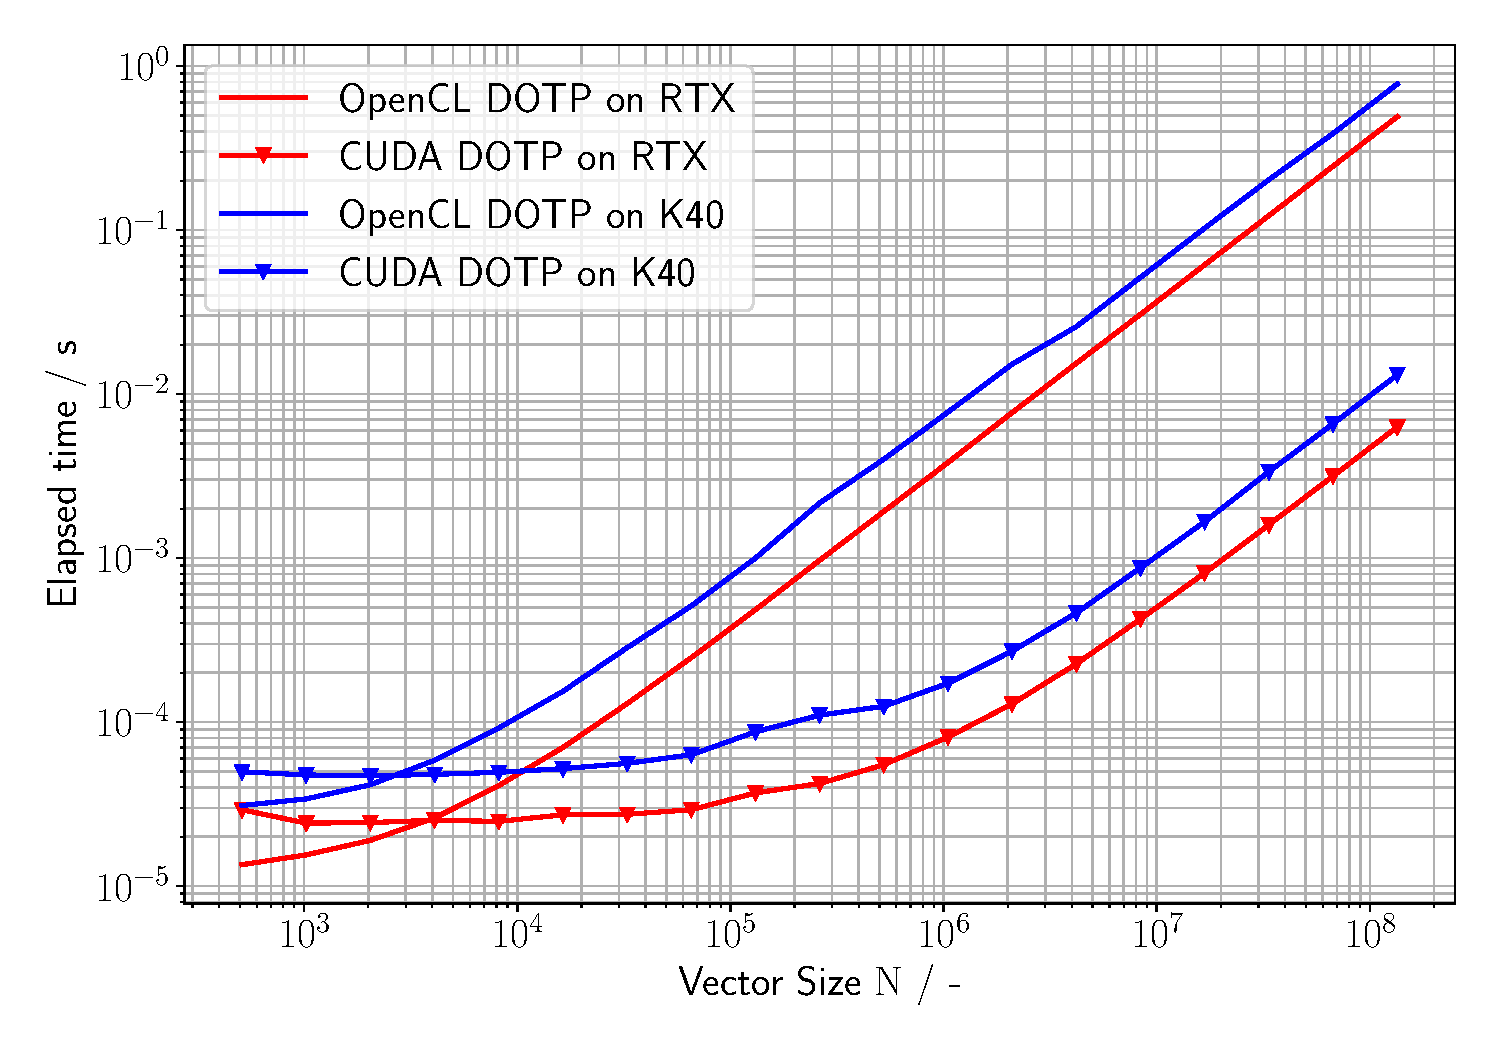
\includegraphics[width = \linewidth]{figures/task_8_2_plot.pdf}
        \caption{Kernel Performance Comparison}
        \end{center}
\end{figure}

\pagebreak
\subsection{Compare Performance of OpenCL Kernels on K40 CPU}
Like mentioned in part 1, here one simply has to change a 0 to a 1 and one can confirm in the output that the CPU is actually used.
CUDA obviously still the fastest. OpenCL Kernel run on K40 is faster than on the CPU.

\begin{figure}[h]
    \begin{center}
        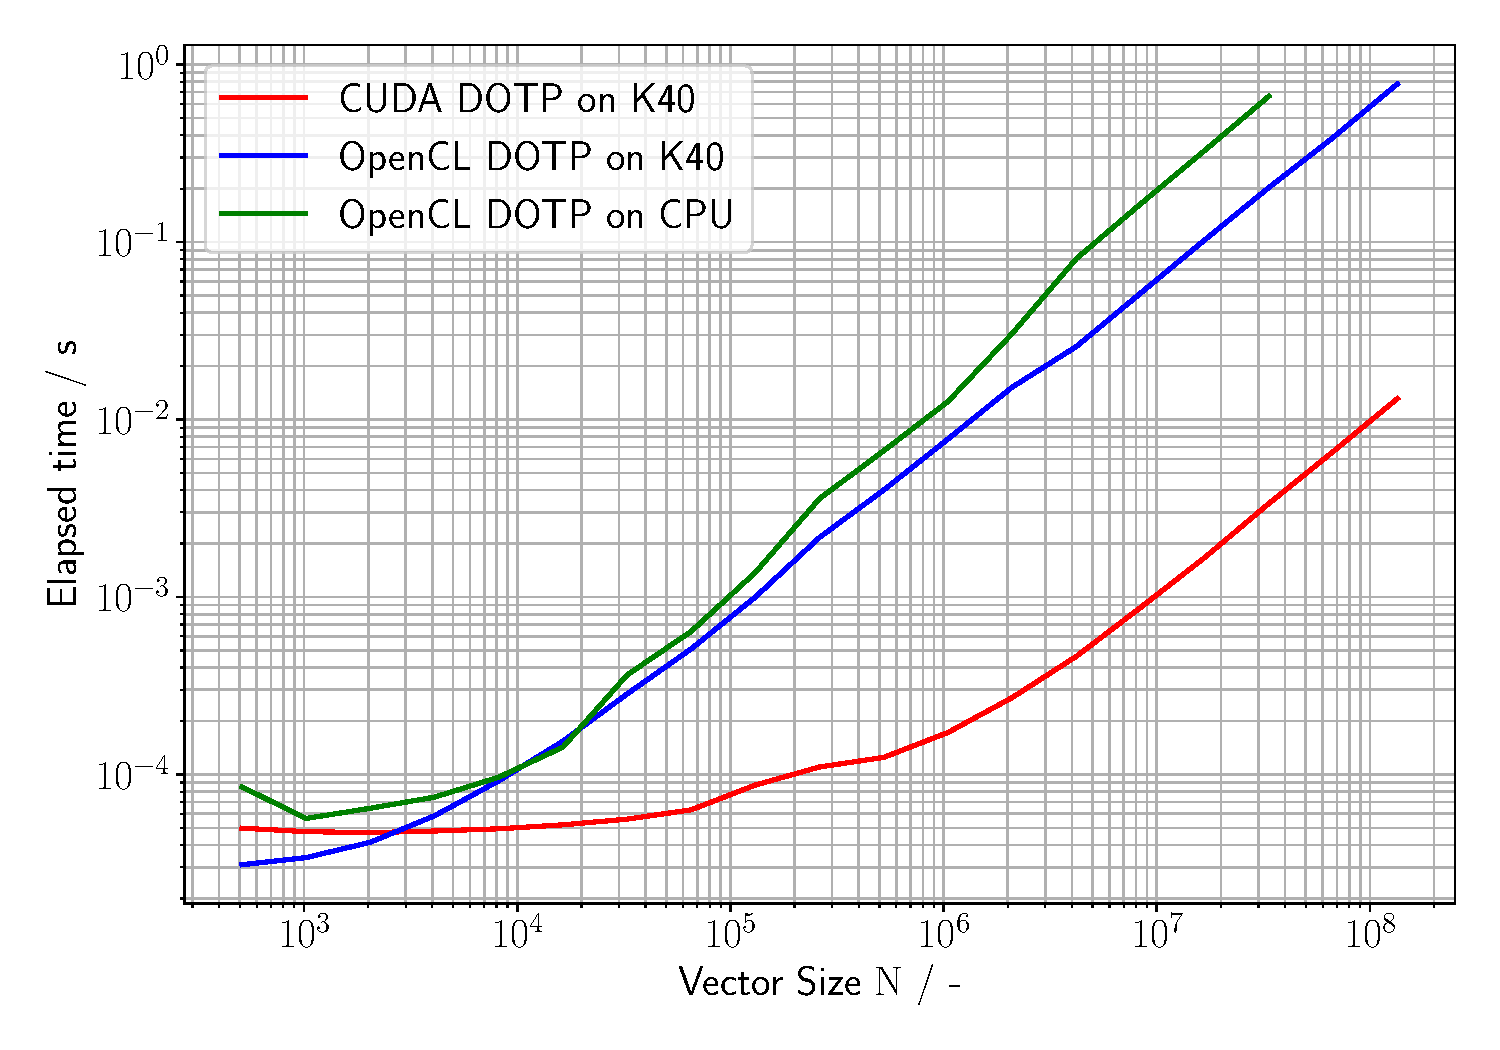
\includegraphics[width = \linewidth]{figures/task_8_3_plot.pdf}
        \caption{CPU GPU performance Comparison}
        \end{center}
\end{figure}
\pagebreak

\subsection{Measure Time it takes to build M OpenCL Programs}
not done :-(.


\pagebreak
\section{Bonus: Implement CUDA+OpenCL (CUCL) Approach (0/1 Points)}
not done :-(.
